\begin{figure*}
\centering
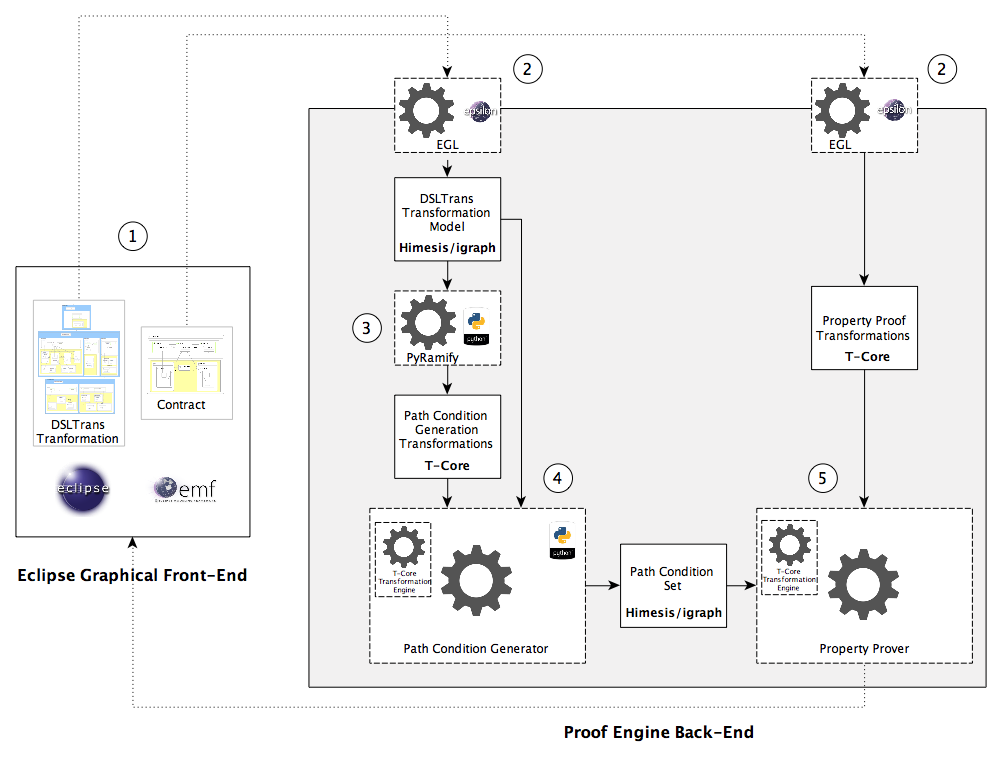
\includegraphics[width=0.8\textwidth]{figures/syvolt_arch}
\caption{The architecture of the SyVOLT tool}
\label{fig:arch}
\end{figure*}

The guiding principle of the Modelling, Design, and Simulation Lab is that all
tools and processes should be explicitly modelled at an appropriate abstraction level.
This practice goes in the direction of ensuring that essential
complexity is the main object of software development and that accidental
complexity is mitigated as much as possible.

SyVOLT's codebase has been developed by applying these principles. We have used
available model-driven development technology as much as possible, both to
develop and as a part of SyVOLT itself. In particular, we have made it such
that the representations of the DSLTrans transformations and the SyVOLT
contracts manipulated by the proof engine are models. The representations of symbolic
executions produced for a given DSLTrans model transformation, also called
\emph{path conditions}, are equally models. Moreover, given the operations
required by the algorithm for building a contract proof (described in~\cite{Lucio2014}) can be implemented as model
manipulations, we have operationally encoded them as model transformations.
In~\cite{LucioVang} how we explain how we use \emph{model transformations to
verify model transformations} in our contract prover.\\

The following model-driven development tools have been used either as part of
SyVOLT's codebase, or for SyVOLT's development:
\begin{itemize}

  \item \textbf{AToM$^3$}~\cite{}: AToM$^3$ is a meta-editor for model-driven
  development. It has been developed at the MSDL and is used for constructing,
  models, metamodels and model transformation rules, and for automatically
  synthesising modeling environments.
  AToM$^3$ has been extensively used to give support to the construction and
  visualisation of models and model transformation rules required by the proof
  engine during the initial stages of the construction of SyVOLT. 
  Many of these artifacts were explicitely built during the construction
  of SyVOLT in order to develop and test the proof algorithm in a controlled
  environment. In the finished SyVOLT all these artifacts are automatically
  generated from their graphical representations in the Eclipse front-end.\\

  \item \textbf{Himesis}~\cite{Provost2006}: Himesis is a typed graph representation
  format, built upon the open-source igraph~\cite{} library. 
Himesis is used for several reasons: independence, efficiency and tool support.
Independence is ensured because Himesis is very expressive and also very simple,
which means it will not change for the foreseeable future.
In \cite{Syriani2010b}, it is reported empirically that Himesis is a good format
to perform the typical graph manipulation operations and it is seamlessly
supported by T-Core.  
  Himesis is used pervasively within SyVOLT to represent models of 
  DSLTrans rules and of SyVOLT contracts, as well as all the model
  transformation rules required by the proof algorithm.\\
  
  \item \textbf{T-Core}~\cite{Syriani2010a}: T-Core is a collection of model transformation
  primitives developed at the MSDL, allowing fine-grained manipulation of
  models. It was initially built as a means to rapidly build
  high-level model transformation languages. T-Core has been used to
  successfully deconstruct and reconstruct several mainstream model transformation
  languages~\cite{}. The main operations of T-Core are model \emph{matching},
  model \emph{rewriting} and \emph{iterating} through a set of match sites in a model.
  The level of control in model manipulation, together with T-Core's speed and
  scalability when treating large models, suited well our needs when
  implementing the property proof algorithm described in~\cite{Lucio2014}. Note that because
  T-Core is also an explicitly modeled model transformation language, a T-Core
  model transformation rule is also a (Himesis) model.\\

  \item \textbf{EMF} (Eclipse Modelling Framework)~\cite{}: SyVOLT makes use of
  EMF's E-Core format for the XMI~\footnote{\url{http://www.omg.org/spec/XMI/}} representation of DSLTrans transformations
  and SyVOLT's contracts within the Eclipse editors. Note that EMF is only used
  in the Eclipse front-end, and that Ecore models are converted into
  the Himesis format for the contract prover engine to compute the
  proofs.\\
  \item \textbf{EGL} (Epsilon Generation Language)~\cite{}: Converting Ecore
  models into Himesis models is achieved using EGL, a language from the Epsilon
  family. Besides easy integration with Eclipse and native support of the expressive
Epsilon Object Language (EOL~\cite{Kolovos}), EGL also provides tasks for the
Ant~\footnote{\url{http://ant.apache.org}} build tool, which was used to
orchestrate the multiple tools in the proving process (see
Section~\ref{sec:push_button_proofs}).\\
\end{itemize}

% Elements of the architecture that could not be built using model driven tools
% (for lack of technological availability) have been developed using model-driven
% principles.

Figure~\ref{fig:arch} shows the architecture of the SyVOLT tool. Two essential
blocks are depicted: the graphical Eclipse front-end and the proof engine
back-end. While the front-end is responsible for the interaction with SyVOLT's
user, the back-end implements the algorithm for running the proofs of the contracts. Note
that two kinds of communication occur between SyVOLT's front-end and back-end:
in the left-to-right direction, a number of artifacts (models and model
transformations) are syntesized from the graphical representations of the
DSLTrans transformations and of the SyVOLT contracts, and passed to the
back-end.
In the reverse direction, the proof result and counter-examples, if any, are
passed from the proof engine back-end to the Eclipse front-end.

Note that in Figure~\ref{fig:arch}, each component is annotated by a number
identifier. Following this numbering sequence, we will briefly visit each
component to describe its function and the technologies employed in its development.

SyVOLT's architectural components described in Figure~\ref{fig:arch} are
orchestrated by an ANT script from within Eclipse. This script makes sure all components execute in the
right order, provides the glue between them and allows contract proof to run at
the push of a button and without any intervention from the part of the user.


% In particular, each artifact and transformation in the contract prover is
% explicitly modelled. EXPAND

% Present:
% \begin{itemize}
%   \item Technology used: introduce orthogonal technologies used in all
%   static components
%   \item Static components
%   \item Flow
% \end{itemize}
% 
% The contract prover makes heavy use of T-Core [CITE], which is a framework of
% transformation primitives. For example, the T-Core Matcher and Rewriter is
% scheduled by Python in order to perform rewriting on a graph in an efficient
% manner.


\subsection{SyVOLT Contract Editor (1)}\levi{too heavy on how it was
developed and tool little on how it is used}

The SyVolt contract editor is realized by a set of Eclipse plugins.
The runtime architecture of this editor is the typical architecture of a
Graphical Modeling Framework (GMF)
\footnote{\url{http://www.eclipse.org/modeling/gmp/}} editor.
What is important is how this editor was developed.

As mentioned in Section~\ref{sec:mdd_gui}, we used Eugenia[CITE] to quickly
develop the SyVolt contract editor shown in Figure~\ref{fig:eclipse_frontend}.

Eugenia consists of a set of annotations that are attached to the metamodel of
SyVOLT contracts. An annotation can, for instance, specify that an atomic
contract will be drawn as a rounded rectangle, with a specific color and a label
that is equal to the name attribute of the contract.
The annotations are not very expressive but they contain the essential
information to generate a set of GMF models that, ultimately, describe a basic
usable graphical editor.

Each generated GMF model is concerned with one aspect of the editor and can be
further customized to our needs. GMF models are much more expressive than the
Eugenia annotations.
For instance, the generated GMF tooling model prescribes the kind of tools that
will be available in the toolbox (shown in the right of
Figure~\ref{fig:eclipse_frontend}), their icons, labels, etc\ldots

From the set of GMF models, a set of eclipse plugins are synthesized.
These make up SyVolt graphical editor\footnote{A fixed structure textual editor
is also provided but this editor lacks several usability improvements and,
hence, is not appropriate to model SyVolt contracts.}.

The original DSLTrans transformation is manipulated using the DSLTrans editor
and is serialized in XMI format. Similarly, SyVOLT contracts are manipulated with the SyVolt graphical
editor and serialized in XMI format.


\subsection{Generating Models and Model Transformations for Proof Construction
(2)}
\label{sec:gen_models_mt}

The translation of DSLTrans transformations and SyVOLT contracts into Himesis
models and model transformation rules was achieved using the Epsilon Generation
Language (EGL~\cite{Rose2008}). More specifically, two EGL model-to-text model
transformations were used: one to generate the Himesis models
representing of a DSLTrans transformation; another one to generate the T-Core
model transformation rules necessary to prove SyVOLT contracts.

These model-to-text transformations are used to parse the Ecore models of a
DSLTrans model transformation under analysis and of the contracts to be proved.
From these Ecore models, the EGL transformations produce a number of Python
files containing classes that inherit from the Himesis library and that
represent models and T-Core transformation rules. These classes are loaded from
disk by the Python interpreter and become models and model transformations in
memory once they are instanciated by the proof engine back-end.
% Note that all these artifacts are produced as
% Python text files containing Himesis format that are needed to automatically
% perform the required proofs.
% containing models of the DSLTrans transformation being analysed
% and the T-Core model transformation rules necessary for the property proof step.

Note that, while this approach of building models and model transformations as
textual files is sufficient for our needs, it is not ideal from the model-driven
development viewpoint. Building models as textual files forces us to deal to
the accidental complexity of Python code and of the Himesis format, making the
generation of these artifacts more difficult and error prone than it needs to
be. The issues encountered here expose one of the current important fragilities
of model-driven development: the difficulty of exchanging high-level data
between different modelling frameworks~\levi{cite benoit combemale here}.


% As opposed to the XMI format which declaratively represents the graph, the
% Himesis representation of a graph is given by Python code referencing the
% Himesis library. When this code is executed it loads the Himesis graph to
% memory.

% Since Himesis is a textual format, identifiers are necessary to correctly
% describe the associations between graph nodes. The EGL transformations make sure
% these are correctly generated.


\subsection{Additional Generation of Model Transformations for Proof
Construction: The PyRamify Script (3)}

Additional model transformations, other than the ones described in
Section~\ref{sec:gen_models_mt}, need to be generated for the property proof
algorithm to execute. These are the \emph{path condition generation} T-Core
model transformations (see Figure~\ref{fig:arch}) that are needed to perform the
model manipulations for building a set of symbolic executions given a DSLTrans
model transformation. These model transformations blocks allow combining the rules of a DSLTrans model
transformation into a set of \emph{path conditions}, as per the algorithm
described in~\cite{Lucio2014}. Note that the path condition generation T-Core
transformations are fully generated from the set of rules of the DSLTrans
transformation being verified.

This additional model transformation generation step is achieved by the PyRamify
component. PyRamify is a Python script that takes as input Himesis graphs
representing the rules in the transformation. Then, through the RAMification
procedure [CITE RAM], T-Core matchers and rewriters for each rule are produced.
Very briefly, while matchers allow the contract prover to determine how
rules might execute over a path condition being built, rewriters properly
combine the right-hand side of a DSLTrans rule with that same path condition
whenever necessary.

% PyRamify is also responsible for producing additional T-Core model
% transformations used for analysing how the DSLTrans rules in a transformation
% depend on each other. Explain this further??

Currently, PyRamify is implemented as a Python script, as we were unable to
implement at the time automatic creation of higher-order artifacts (in our
case, T-Core transformations) from models in another modelling tool.
This was due to the mix of different modelling abstraction levels present in
SyVOLT and that led to a number of technical difficulties.

We have recently learned that, alternatively, \emph{path condition generation
transformations} could be built directly from the Ecore representation of
DSLTrans rules by using EGL technology -- as was done for the artifacts
described in Section~\ref{sec:gen_models_mt}. Nevertheless, a preferred solution for us would
be to use model transformation technology that that explicitely allows
building model transformations from simple models. To the best of our knowledge,
model transformation technology that allows moving between models of an order 
$n$ and an order $n+1$ is not yet available in the modelling community.

\subsection{Path Condition Generation (4)}
\label{sec:path_cond_gen}

Once the required artifacts have been produced, the prover moves onto the path
condition generation step. Each path condition will represent an (infinite) set
of concrete executions of the transformation, where each concrete execution is an
input/ouput pair. Path condition generation is operationally achieved by
executing, following the ordering of the rules in the DSLTrans
tranformation being analysed, the \emph{path condition generation transformations} generated by the
\emph{PyRamify} component. 

The path condition generation algorithm starts from the empty path condition,
representing the case where no rules in the transformation have executed. Then,
as each T-Core transformation in the \emph{path condition generation
transformations} set is executed, each rule in the DSLTrans model transformation
under analysis is combined with the path conditions generated thus far. As each
rule is considered, the set of path conditions will grow
to represent all allowed combinations rules combinations. As the execution of a
rule in a DSLTrans transformation may depend on the previous execution of other rules,
such dependencies are verified by the \emph{path condition generation
transformations} in order to exclude impossible rule combinations.

% The final set of path conditions produced by the algorithm will then abstract
% the infinite set of all concrete transformation executions. This is further
% described in~\cite{Lucio2014}, along with a formal discussion of the validity
% and completeness of this work.

Note that \emph{path condition generation} is a complex task, difficult to fully
model as a single model transformation. As such, the algorithm
has been implemented as a Python script that is responsible for scheduling all the
\emph{path condition generation transformations} in the right order. This programmatic level of granularity of
manipulation has allowed us to build many optimizations to speed up the path
condition generation process. Examples of such optimizations are the caching of
expensive match operations, or the parallelization of the path condition generation algorithm. 

\subsection{Contract Proof (5)}

Once the path conditions are generated, the proof that each
contract holds or does not hold can then be built. The \emph{contract proof}
component requires two inputs: the \emph{path conditions set} built by the path
condition generator; the \emph{property proof T-Core transformations}, generated by EGL model-to-text
transformations as described in Section~\ref{sec:gen_models_mt}.

Pre- / post- condition contracts form an implication, which needs to be
checked for each path condition provided as input to the contract proof
component. For a contract to hold on a DSLTrans model transformation, the
contract's implication should hold for every path condition generated for
that model transformation. Checking if the implication between a contract's pre-
and post- condition holds on a path condition is achieved by attempting to find for each submodel of
the path condition that is isomorphic to the pre-condition's model, a submodel
of the path condition that is isomorphic to the post-condition's model. The
computations on the existence of these sugraphs isomorphisms is done by
the \emph{T-Core property proof transformations}. Note that, in this case, the
T-Core transformations are simply a set of matchers, or queries, as no further
editing of the path conditions is necessary during this part of the proof.

As in for the path condition generation component described in
Section~\ref{sec:path_cond_gen}, the contract proof algorithm has also been
implemented as a Python script that schedules all the property proof T-Core
transformations appropriately. As before, using fine-grained programmatic
manipulations of the models and model transformations involved in the contract
proof algorithm has allowed us to implement optimization strategies. The main
of these strategies is the skipping of path conditions for which the contract
is sure to hold without further analysis, given existing cached information
about similar path conditions.


